\documentclass[a4paper]{article}

%------------------------------------------------------------
\usepackage[a4paper, total={6in, 9in}]{geometry}
\usepackage{amsmath, amssymb}
\usepackage{booktabs}
\usepackage{caption}
\usepackage{enumitem}
\usepackage{graphicx}
\usepackage{float}
\usepackage{inconsolata}
\usepackage{listings}
\usepackage{mathtools}
\usepackage{pstricks-add}
\usepackage{siunitx}
\usepackage[most]{tcolorbox}
\usepackage{tikz, pgfplots}
\usepackage{epstopdf} %converting to PDF
\usepackage{hyperref}
\usepackage{xfrac}

\usetikzlibrary{shapes.geometric}
\usetikzlibrary{arrows}
\usetikzlibrary{calc}

%------------------------------------------------------------
\graphicspath{{./fig/}}
\pgfplotsset{compat=1.13}
%------------------------------------------------------------
\setlength{\parindent}{0in}

\lstdefinestyle{C++}{
	language=C++,
	basicstyle=\ttfamily,
	keywordstyle=\color{blue}\ttfamily,
	stringstyle=\color{red}\ttfamily,
	commentstyle=\color{green}\ttfamily,
	morecomment=[l][\color{magenta}]{\#},
	showstringspaces=false
}

%------------------------------------------------------------
\newtcblisting[auto counter]{sexylisting}[2][]{sharp corners, 
    fonttitle=\bfseries, colframe=gray, listing only, 
    listing options={basicstyle=\ttfamily,language=C++}, 
    title=Listing \thetcbcounter: #2, #1}

%------------------------------------------------------------
\lstset{language=C++,
        basicstyle=\ttfamily,
        keywordstyle=\color{blue}\ttfamily,
        stringstyle=\color{red}\ttfamily,
        commentstyle=\color{green}\ttfamily,
        morecomment=[l][\color{magenta}]{\#},
        showstringspaces=false
}
%------------------------------------------------------------
\tikzstyle{block} = [draw, fill=blue!20, rectangle, 
    minimum height=3em, minimum width=3em]
\tikzstyle{sum} = [draw, fill=blue!20, circle, node distance=1cm]
\tikzstyle{input} = [coordinate]
\tikzstyle{output} = [coordinate]
\tikzstyle{pinstyle} = [pin edge={to-,thin,black}]

%------------------------------------------------------------
\newlength{\arrow}
\settowidth{\arrow}{\scriptsize$1000$}

\newcommand*{\myrightarrow}[1]{\xrightarrow{\mathmakebox[\arrow]{#1}}}

\newcommand{\uvec}[1]{\boldsymbol{\hat{\textbf{#1}}}}

%------------------------------------------------------------

\begin{document}
\title{ENG252 Dynamics: Practical 3}
\author{Shane Reynolds}
\maketitle

\section{Introduction}
Consider a body with mass $m$ undergoing rotational motion, with angular acceleration $\alpha$, around a fixed axis $OO'$. Graphically this scenario is depicted in Figure 1. If we want to calculate the Moment of this body around the axis $OO'$, then we need to consider the moments of each and every infinitesimally small mass particle that make up the body. The moment of a single particle mass is given by:
\begin{equation}
M = \boldsymbol{r} \times \boldsymbol{F}
\end{equation}

We note $\boldsymbol{r}$ is the position vector of the particle from point where the moment is to calculated, and $\boldsymbol{F}$ is the force acting on the particle. If our motion is constrained to a 2D plane, equation (1) simplifies to the well known equation:
\begin{equation}
M = F \times d
\end{equation}
The quantity $F$ is the scalar magnitude of the force acting orthogonal to the shortest line connecting the particle mass to the moment point of calculation; and $d$ is the distance between between these two points. Using (2) we can calculate the moment $M_O$ about axis $OO'$ for a small mass element, $dm$, of the body in Figure 1:
\begin{equation}
	M_O = Fr = a_t \ dm \ r 
\end{equation}

\begin{figure}[h]
	\centering
	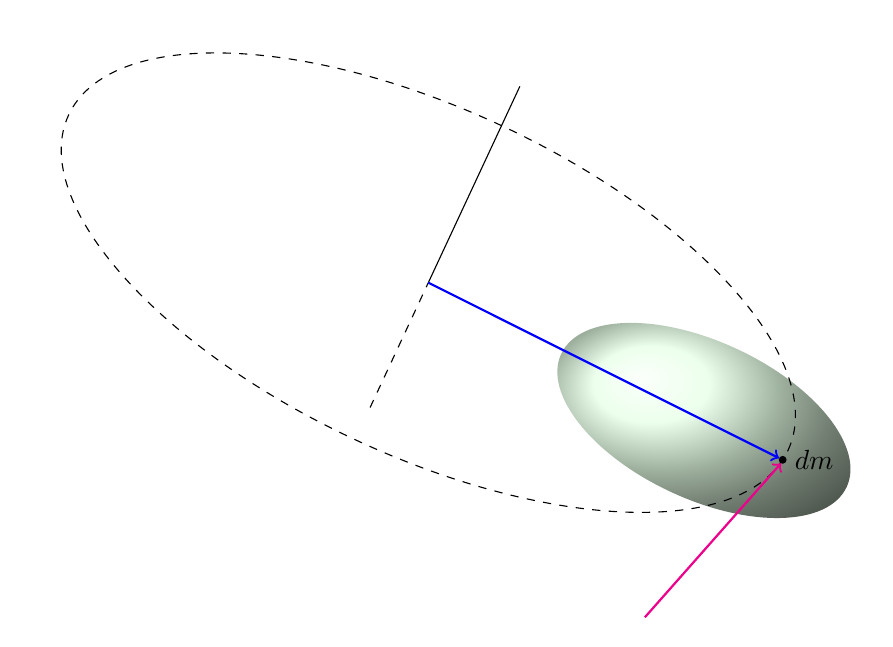
\begin{tikzpicture}
		\shade[ball color=green!10!, rotate=-25] (0,0) coordinate(C) ellipse (2 and 1);
		\fill[color=black] (1,-0.5) circle (0.05); 
		\draw[rotate around={-25:(-3.5,1.75)}] (-3.5,1.75) -- (-3.5,4.5);
		\draw[dashed, rotate around={-25:(-3.5,1.75)}] (-3.5,0) -- (-3.5,1.75);
		\draw[->, color=blue, thick] (-3.5,1.75) -- (0.9546,-0.4788);
		\draw [dashed, rotate around={-25:(-3.5,1.75)}] (-3.5,1.75) ellipse (5.04 and 2.2);
		\draw [->, color=magenta, thick] (-0.75,-2.5) -- (0.9788,-0.545);
		\node at (1.4,-0.5) {$dm$};
	\end{tikzpicture}
	\caption{A body of mass $m$ rotating about a fixed axis $OO'$ with some angular acceleration $\alpha$.}
\end{figure}

According to Giancoli a particle undergoing fixed axis rotation can re-express tangential acceleration $a_t$, as $\alpha r$, where $r$ is the distance from the centre of rotation to the particle. We can now rite (3) as:
\begin{equation}
M_O = \alpha r \ dm \ r
\end{equation}

This is convenient since $\alpha$ remains constant for all infinitesimally small particles in the body meaning that the only variable that needs consideration is $r$. In fact, to calculate the sum of the moments of the body around axis $OO'$ we need to integrate the right hand side of equation (4), which yields:
\begin{equation}
\sum M_O = \alpha \int r^2 dm
\end{equation}

Equation (5) is often thought of as somewhat analogous to $\sum F = ma$, but for rotational motion. In fact since $\alpha$ is the angular acceleration, the integral in equation (5) is often referred to as the resistance of a body to change it's state of rotation. In the literature this quantity is denoted $I_O$ and referred to as the Moment of Inertia and is defined as:
\begin{equation}
I = \int r^2 dm
\end{equation}

\begin{figure}[h]
	\centering
	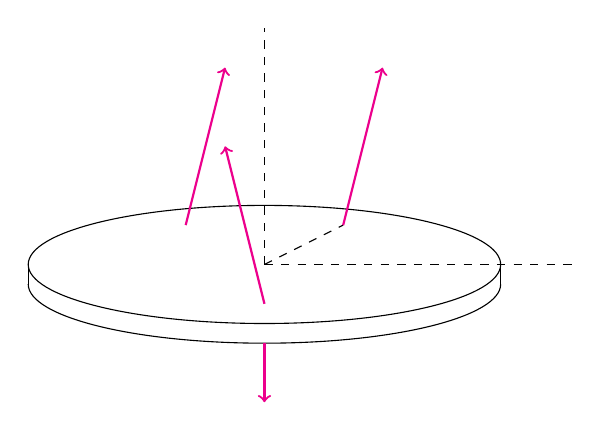
\begin{tikzpicture}
		\draw (0,0) ellipse (3 and 0.75);
		\draw (-3,-0.25) arc (180:360:3 and 0.75);
		\draw (-3,0) -- (-3,-0.25);
		\draw (3,0) -- (3,-0.25);
		\draw [dashed] (0,0) -- (0,3);
		\draw [dashed] (0,0) -- (4,0);
		\draw [dashed] (0,0) -- (1,0.5);
		\draw [->, thick, color=magenta] (1,0.5) -- (1.5,2.5);
		\draw [->, thick, color=magenta] (-1,0.5) -- (-0.5,2.5);
		\draw [->, thick, color=magenta] (0,-0.5) -- (-0.5, 1.5);
		\draw [->, thick, color=magenta] (0,-1) -- (0, -1.75);
	\end{tikzpicture}
\end{figure}

\begin{figure}[h]
	\centering
	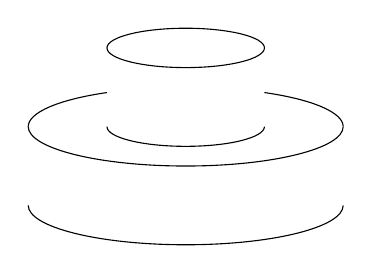
\begin{tikzpicture}
		\draw (0,0) ellipse (1 and 0.25);
		\draw (-1,-1) arc (180:360:1 and 0.25);
		\draw (-2,-1) arc (180:360:2 and 0.5);
		\draw (-2,-1) arc (180:240:2 and -0.5);
		\draw (2,-1) arc (360:300:2 and -0.5);
		\draw (-2,-2) arc (180:360:2 and 0.5);
	\end{tikzpicture}
\end{figure}

\begin{figure}[h]
	\centering
	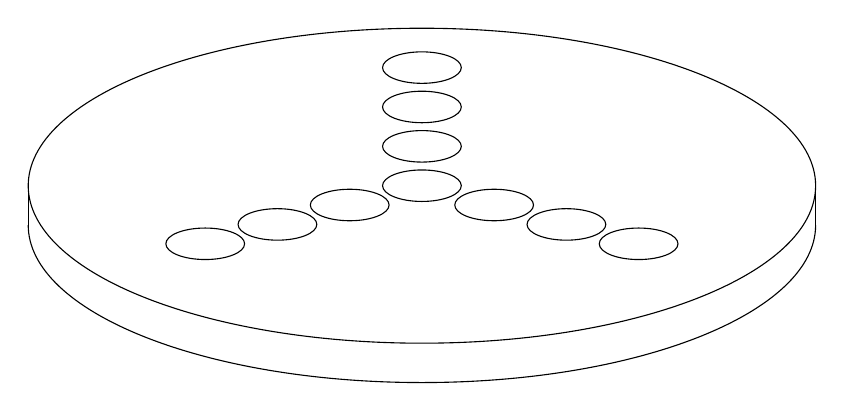
\begin{tikzpicture}
		\draw (0,0) ellipse (5 and 2);
		\draw (-5,-0.5) arc (180:360:5 and 2);
		\draw (-5,0) -- (-5,-0.5);
		\draw (5,0) -- (5,-0.5);
		
		\draw (0,0) ellipse (0.5 and 0.2);
		
		\draw (0,0.5) ellipse (0.5 and 0.2);
		\draw (0,1) ellipse (0.5 and 0.2);
		\draw (0,1.5) ellipse (0.5 and 0.2);
		
		\draw (-0.917,-0.245) ellipse (0.5 and 0.2);
		\draw (-1.835,-0.4917) ellipse (0.5 and 0.2);
		\draw (-2.752,-0.7376) ellipse (0.5 and 0.2);
		
		\draw (0.917,-0.245) ellipse (0.5 and 0.2);
		\draw (1.835,-0.4917) ellipse (0.5 and 0.2);
		\draw (2.752,-0.7376) ellipse (0.5 and 0.2);
	\end{tikzpicture}
\end{figure}



Talk about rotational inertia

Talk about derivation because atan = alpha times r

Talk about the analogous nature to f = ma

Talk about mass moments of inertia and how to calculate

Talk about radius of gyration



\subsection{Scope}

\section{Results}

\section{Calculations}

\begin{figure}[h]
	\centering
	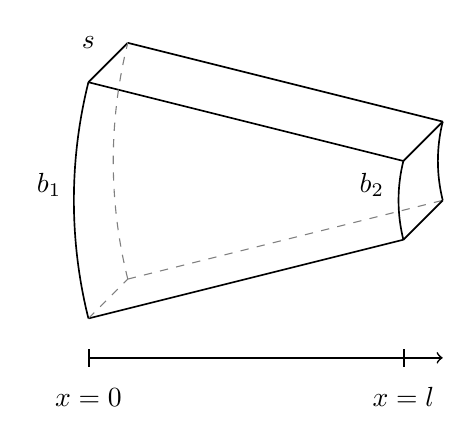
\begin{tikzpicture}
	% general shift to north east
	\coordinate (O) at (0.5,0.5);
	\draw[semithick] (0,0) -- (4,1);% bottom line in front
	\draw[dashed,color=gray] (O) -- ($(4,1)+(O)$);% bottom line in the back
	\draw[semithick] (0,3) -- (4,2);% top line in front
	\draw[semithick] ($(0,3)+(O)$) -- ($(4,2)+(O)$);% top line in the back
	\draw[semithick] (0,3) -- ($(0,3)+(O)$);% line to the back, top left
	\draw[semithick] (4,2) -- ($(4,2)+(O)$);% line to the back, top right
	\draw[semithick] (4,1) -- ($(4,1)+(O)$);% line to the back, bottom right
	\draw[dashed,color=gray] (0,0) -- (O);% line to the back, bottom left
	% the first angle is 180°+atan(0.25)
	% the second angle is 180°-atan(0.25)
	% the radius is sqrt(6^2+1.5^2)
	\draw[semithick] (0,0) arc (194.036:165.964:6.185);% left arc in front
	\draw[dashed,color=gray] (O) arc (194.036:165.964:6.185);% left arc in the back
	% the first angle is 180°+atan(0.25)
	% the second angle is 180°-atan(0.25)
	% the radius is 1/3*sqrt(6^2+1.5^2)
	\draw[semithick] (4,1) arc (194.036:165.964:2.062);% right arc in front
	\draw[semithick] ($(4,1)+(O)$) arc (194.036:165.964:2.062);% right arc in the back
	\draw (-0.5,1.7) node {$b_1$};
	\draw (3.6,1.7) node {$b_2$};
	\draw (0,3.5) node {$s$};
	\draw[|-,semithick] (0,-0.5) -- (4,-0.5);
	\draw[|->,semithick] (4,-0.5) -- (4.5,-0.5);
	\draw (0,-1) node {$x=0$};
	\draw (4,-1) node {$x=l$};
	\end{tikzpicture}
\end{figure}

\section{Discussion}

\section{Conclusion}


\bibliography{my_bib}
\bibliographystyle{ieeetr}

\end{document}